\documentclass[11pt,a4paper]{article}

\usepackage[margin=2.3cm]{geometry}
\usepackage[T1]{fontenc}
\usepackage{lmodern}
\usepackage{amsmath,amssymb,amsthm,mathtools,bm}
\usepackage{booktabs,tabularx,array,longtable}
\usepackage{hyperref}
\usepackage{enumitem}
\usepackage{xcolor}
\usepackage{listings}
\usepackage{tikz}
\usepackage{microtype}
\usetikzlibrary{arrows.meta,positioning,calc}

\hypersetup{colorlinks=true,linkcolor=blue!60!black,urlcolor=blue!60!black}

\theoremstyle{definition}
\newtheorem{definition}{Definition}
\newtheorem{proposition}{Proposition}
\newtheorem{remark}{Remark}

\newcommand{\Her}{\operatorname{Her}}
\newcommand{\jomega}{\mathrm{j}\omega}
\newcommand{\CC}{\mathbb{C}}
\newcommand{\RR}{\mathbb{R}}
\newcommand{\code}[1]{\texttt{\detokenize{#1}}}

\lstset{
  basicstyle=\ttfamily\footnotesize,
  frame=single,
  breaklines=true,
  breakatwhitespace=false,
  columns=fullflexible,
  keepspaces=true,
  showstringspaces=false,
  aboveskip=0.6em,
  belowskip=0.6em,
  xleftmargin=0.5em,
  xrightmargin=0.5em,
  literate={*}{{\char42}}1
}

\newcolumntype{L}[1]{>{\raggedright\arraybackslash}p{#1}}
\newcolumntype{Y}{>{\raggedright\arraybackslash}X}

\tikzset{
  Fbox/.style={draw, rounded corners=2pt, align=center, font=\small,
               text width=9.2cm, minimum height=0.72cm, inner sep=3pt,
               anchor=west},
  Ftag/.style={draw, rounded corners=2pt, font=\scriptsize\bfseries,
               minimum width=1.7cm, minimum height=0.55cm, inner sep=2pt,
               anchor=west},
  Narr/.style={-{Latex}, thick},
  ColA/.style={draw, rounded corners=2pt, align=center, font=\scriptsize,
               text width=3.5cm, minimum height=0.65cm, inner sep=3pt, fill=blue!10},
  ColB/.style={draw, rounded corners=2pt, align=center, font=\scriptsize,
               text width=3.5cm, minimum height=0.65cm, inner sep=3pt, fill=orange!12}
}

\title{\textbf{Harmony Certificate Layer}\\
\large Mathematical Reference, Implementation Map, and Expansion Roadmap}
\author{Companion notes for the Harmony toolbox\\
Track~B = Leki\'c--Beerten impedance method ($H=YZ_{\mathrm{eq}}$)\\
\code{src/Solver/Certificate/} + \code{StabilityEstimate} + MMC}
\date{\today}

\begin{document}
\maketitle

\begin{abstract}
These notes document what Harmony's certificate layer computes today,
how it sits on the \textbf{Leki\'c--Beerten} impedance pipeline
($Y$, $Z_{\mathrm{eq}}$, $H=YZ_{\mathrm{eq}}$), and what remains relative to full
compositional DW/SRG interconnection theorems. Local \textbf{geometric certificates}
(numerical range, small-gain, DW-lite shell, sector/loop-shift) are implemented in
\code{Geometric_certificates.*}. Formulas, workflows, distinctive test cases,
and how to run the unit/demo tests are included.
\end{abstract}

\tableofcontents
\newpage

%==============================================================================
\section{Ownership of the two tracks}
%==============================================================================

\begin{center}
\renewcommand{\arraystretch}{1.25}
\begin{tabularx}{\textwidth}{@{}L{0.46\textwidth} Y@{}}
\toprule
\textbf{Track B --- Impedance / return ratio} &
\textbf{Track A --- Local geometric certificates} \\
\midrule
$Y(\jomega)$, $Z_{\mathrm{eq}}$, $H=YZ_{\mathrm{eq}}$, MIMO Bode/Nyquist.
\textbf{Leki\'c--Beerten line} (author home turf).
First-class in Harmony (\code{StabilityEstimate}).
&
Passivity, eigenphase, numerical-range (small-phase), small-gain,
excess/shortage, DW-lite shell, sector/loop-shift, PnP gate.
\textbf{Local sufficient screens}, not a full compositional DW/SRG
network theorem. \\
\bottomrule
\end{tabularx}
\end{center}

\vspace{0.4em}
Narrative: extend the $H$-based MMC--HVDC platform with modern local geometric
certificates, and measure their conservatism against your own $H$ --- not
``reimplement ETH theory.''

%==============================================================================
\section{Pipeline vs Harmony today}
%==============================================================================

\begin{center}
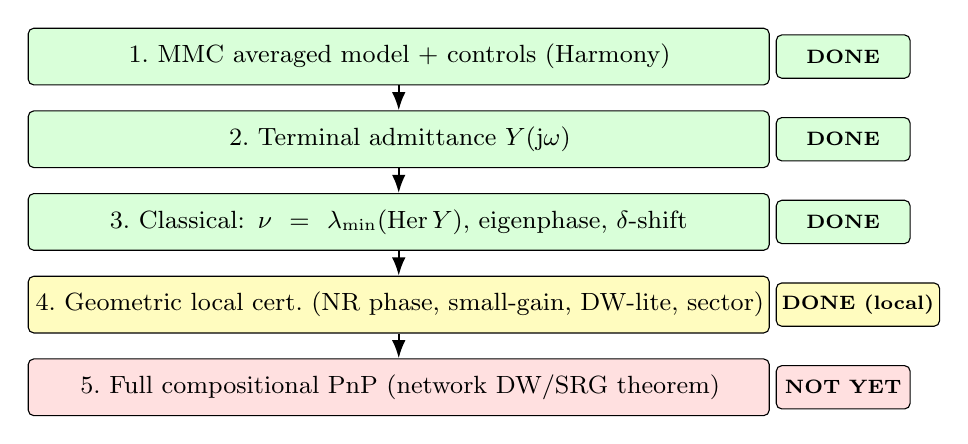
\begin{tikzpicture}
  \node[Fbox, fill=green!15] (a) at (0,0)
    {1.\ MMC averaged model + controls (Harmony)};
  \node[Ftag, fill=green!15] (ta) at (9.5,0) {DONE};

  \node[Fbox, fill=green!15] (b) at (0,-1.05)
    {2.\ Terminal admittance $Y(\jomega)$};
  \node[Ftag, fill=green!15] (tb) at (9.5,-1.05) {DONE};

  \node[Fbox, fill=green!15] (c) at (0,-2.1)
    {3.\ Classical: $\nu=\lambda_{\min}(\Her Y)$, eigenphase, $\delta$-shift};
  \node[Ftag, fill=green!15] (tc) at (9.5,-2.1) {DONE};

  \node[Fbox, fill=yellow!25] (d) at (0,-3.15)
    {4.\ Geometric local cert.\ (NR phase, small-gain, DW-lite, sector)};
  \node[Ftag, fill=yellow!25] (td) at (9.5,-3.15) {DONE (local)};

  \node[Fbox, fill=red!12] (e) at (0,-4.2)
    {5.\ Full compositional PnP (network DW/SRG theorem)};
  \node[Ftag, fill=red!12] (te) at (9.5,-4.2) {NOT YET};

  \draw[Narr] (a.south)--(b.north);
  \draw[Narr] (b.south)--(c.north);
  \draw[Narr] (c.south)--(d.north);
  \draw[Narr] (d.south)--(e.north);
\end{tikzpicture}
\end{center}

Network assessment today uses Track~B in parallel: $H=YZ_{\mathrm{eq}}$
(Bode/Nyquist) plus optional $\Her(I+H)$ proxy.

\begin{center}
\renewcommand{\arraystretch}{1.15}
\begin{tabularx}{\textwidth}{@{}L{2.6cm} Y L{2.8cm}@{}}
\toprule
Step & In Harmony & Status \\
\midrule
MMC model & Averaged MMC + ABCD + GFM & Done \\
$Y(s)$ & \code{compute_y_parameters} & Done \\
Classical screens & $\nu$, eigenphase, $\delta$-shift & Done \\
Geometric local & NR, small-gain, DW-lite, sector & Done (local) \\
Network check & $H=YZ_{\mathrm{eq}}$ (+ $\Her(I+H)$) & Done (impedance) \\
Compositional PnP & Network DW/SRG theorem & Missing \\
\bottomrule
\end{tabularx}
\end{center}

%==============================================================================
\section{Two parallel tracks}
%==============================================================================

\begin{center}
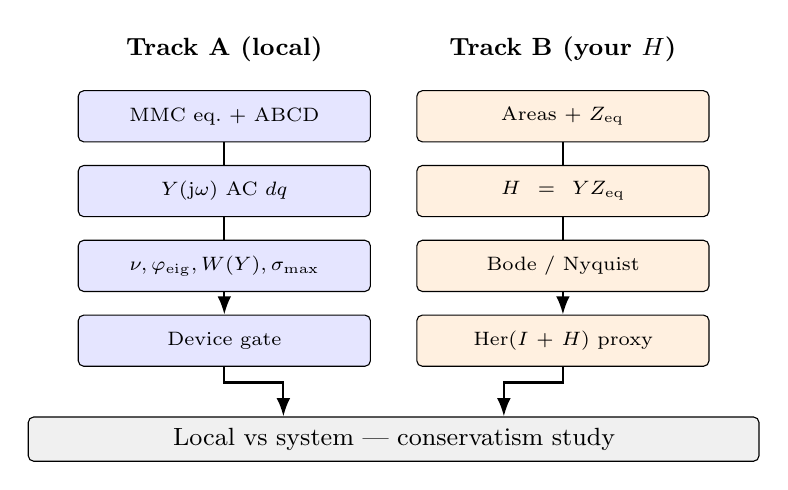
\begin{tikzpicture}
  \node[font=\small\bfseries] at (-2.15,0.85) {Track A (local)};
  \node[font=\small\bfseries] at (2.15,0.85) {Track B (your $H$)};

  \node[ColA] (a1) at (-2.15,0) {MMC eq.\ + ABCD};
  \node[ColA] (a2) at (-2.15,-0.95) {$Y(\jomega)$ AC $dq$};
  \node[ColA] (a3) at (-2.15,-1.9) {$\nu,\varphi_{\mathrm{eig}},W(Y),\sigma_{\max}$};
  \node[ColA] (a4) at (-2.15,-2.85) {Device gate};

  \node[ColB] (b1) at (2.15,0) {Areas + $Z_{\mathrm{eq}}$};
  \node[ColB] (b2) at (2.15,-0.95) {$H=YZ_{\mathrm{eq}}$};
  \node[ColB] (b3) at (2.15,-1.9) {Bode / Nyquist};
  \node[ColB] (b4) at (2.15,-2.85) {$\Her(I+H)$ proxy};

  \node[draw, rounded corners=2pt, fill=gray!12, align=center, font=\small,
        text width=9.0cm, inner sep=4pt] (c) at (0,-4.1)
    {Local vs system --- conservatism study};

  \draw[Narr] (a1)--(a2)--(a3)--(a4);
  \draw[Narr] (b1)--(b2)--(b3)--(b4);
  \draw[Narr] (a4.south) -- ++(0,-0.2) -| ([xshift=-1.4cm]c.north);
  \draw[Narr] (b4.south) -- ++(0,-0.2) -| ([xshift=1.4cm]c.north);
\end{tikzpicture}
\end{center}

\noindent\textbf{Code map.}
\code{Geometric_certificates}, \code{Stability_certificate},
\code{Device_gate}, \code{PnP_library}, \code{Operating_region},
\code{Tuning_assistant}, \code{Local_vs_system}, \code{StabilityEstimate}.
Demo: \code{Harmony --cpp certificate_figures}.

%==============================================================================
\section{Plant, linearization, admittance}
%==============================================================================

\subsection{Equilibrium and ABCD}
\[
  \dot x=f(x,u),\quad y=g(x,u),\qquad f(x^\star,u^\star)=0,
\]
\[
  \Delta\dot x=A\Delta x+B\Delta u,\qquad
  \Delta y=C\Delta x+D\Delta u.
\]

\subsection{Admittance}
\[
  Y(s)=C(sI-A)^{-1}B+D,\qquad s=\jomega.
\]

\subsection{MMC multiport}
\[
  Y=\begin{bmatrix} Y_{\mathrm{dd}} & Y_{\mathrm{da}}\\ Y_{\mathrm{ad}} & Y_{\mathrm{aa}}\end{bmatrix},
  \qquad
  Y_{\mathrm{ac}}:=Y_{\mathrm{aa}}\in\CC^{2\times 2}
\]
(default: \code{ac_dq_block=true}).

\begin{remark}[Methodological home]
Forming $Y(\jomega)$ and assessing interconnection via $H=YZ_{\mathrm{eq}}$
is the Leki\'c--Beerten impedance workflow (Track~B).
\end{remark}

%==============================================================================
\section{Classical metrics}
%==============================================================================

\[
  \Her(Y)=\tfrac{1}{2}(Y+Y^*),\qquad
  \nu(Y)=\lambda_{\min}(\Her Y),\qquad
  \nu_\delta(Y)=\lambda_{\min}\bigl(\Her(Y+\delta I)\bigr).
\]
\[
  \varphi_{\mathrm{eig}}(Y)
  =\max_{i:\,\lambda_i\neq 0}\lvert\arg\lambda_i(Y)\rvert
  \quad\text{(heuristic eigenphase)}.
\]
Excess / shortage:
\[
  \nu_+(Y)=\max\bigl(0,\nu(Y)\bigr),\qquad
  \nu_-(Y)=\max\bigl(0,-\nu(Y)\bigr).
\]
Log-grid $f_k$; worst-case aggregates over the sweep.
ALLOW iff all enabled checks in \code{CertificateSpec} pass
(\code{sweepPassesSpec}).

%==============================================================================
\section{Geometric certificates (implemented)}
%==============================================================================

Module: \code{Geometric_certificates.h/.cpp}. Metrics are always written into
each \code{CertificateSweep}; enforcement is opt-in via \code{require_*} flags.

\subsection{Numerical range (field of values)}
\[
  W(Y)=\{v^*Yv:\|v\|=1\}\subset\CC.
\]
Support-function boundary
\[
  z(\theta)=e^{\mathrm{j}\theta}\,
  \lambda_{\max}\!\bigl(\Her(e^{-\mathrm{j}\theta}Y)\bigr),\qquad
  \theta\in[0,2\pi).
\]
\begin{itemize}[leftmargin=*,itemsep=0.2em]
  \item $\displaystyle\min\operatorname{Re} W(Y)=\nu(Y)$.
  \item \textbf{NR phase:}
        $\displaystyle
        \varphi_{\mathrm{NR}}(Y)
        =\max_{z\in\partial W(Y)}\lvert\arg z\rvert$
        (set to $180^\circ$ if $0\in W(Y)$).
  \item \textbf{Zero margin:}
        $\displaystyle
        m_0(Y)=-\min_\theta\lambda_{\max}\bigl(\Her(e^{-\mathrm{j}\theta}Y)\bigr)$.
        Then $m_0>0\Rightarrow 0\notin W$; $m_0\le 0\Rightarrow 0\in W$
        (dense $\theta$-grid).
\end{itemize}
Flags: \code{require_nr_phase}, \code{require_nr_zero_outside}.

\subsection{Small-gain}
\[
  \sigma_{\max}(Y)=\|Y\|_2,\qquad
  \text{pass if }\sigma_{\max}(Y)\le\gamma.
\]
Flags: \code{require_small_gain}, \code{gain_limit}$=\gamma$.

\subsection{Davis--Wielandt shell (DW-lite, local)}
\[
  \mathrm{DW}(Y)
  =\bigl\{\bigl(v^*Yv,\|Yv\|^2\bigr):\|v\|=1\bigr\}
  \subset\CC\times\RR_+.
\]
Harmony samples $\mathrm{DW}(Y)$ and plots the xz projection
$(\operatorname{Re}(v^*Yv),\|Yv\|^2)$. Local DW-lite gate (\code{require_dw}):
\[
  0\notin W(Y)\quad\text{and}\quad
  \varphi_{\mathrm{NR}}(Y)\le\varphi_{\mathrm{lim}}.
\]
\begin{remark}[Honesty]
Local geometric screen only --- not the ETH projected-shell SDP /
converter--network DW separation theorem.
\end{remark}

\subsection{Sector / loop-shift}
For sector $[\alpha,\beta]$ with $\beta>\alpha$,
\[
  T=(Y-\alpha I)(\beta I-Y)^{-1}
\]
(when invertible). Sector certificate: $\nu(T)\ge\varepsilon$
(\code{require_sector}, \code{sector_alpha}, \code{sector_beta}).

\subsection{Spec flags}
\begin{center}
\renewcommand{\arraystretch}{1.1}
\begin{tabularx}{\textwidth}{@{}L{4.4cm} Y@{}}
\toprule
Flag & Enforces \\
\midrule
\code{require_passivity} & $\nu_{\mathrm{worst}}\ge\varepsilon$ \\
\code{require_phase} & $\varphi_{\mathrm{eig,worst}}\le\varphi_{\mathrm{lim}}$ \\
\code{require_shifted} & $\nu_{\delta,\mathrm{worst}}\ge\varepsilon$ \\
\code{require_nr_phase} & $\varphi_{\mathrm{NR,worst}}\le\varphi_{\mathrm{lim}}$ \\
\code{require_nr_zero_outside} & $m_{0,\mathrm{worst}}>0$ \\
\code{require_small_gain} & $\sigma_{\max,\mathrm{worst}}\le\gamma$ \\
\code{require_dw} & DW-lite (zero-out + NR phase) \\
\code{require_sector} & loop-shifted sector passivity \\
\bottomrule
\end{tabularx}
\end{center}

%==============================================================================
\section{Track B: return ratio}
%==============================================================================

\[
  H(\jomega)=Y_{\mathrm{conv}}(\jomega)\,Z_{\mathrm{eq}}(\jomega).
\]
Optional proxy:
\[
  \nu_{\mathrm{sys}}(\omega)=\lambda_{\min}\bigl(\Her(I+H(\jomega))\bigr).
\]
Classical assessment remains Bode/Nyquist of $H$. Consistency:
\[
  \mathrm{consistent}\iff(\mathrm{local\_pass}=\mathrm{system\_pass}).
\]
GFM-MMC often: local FAIL, system PASS --- seed for non-passivity bands.

%==============================================================================
\section{Five workflows}
%==============================================================================

\begin{center}
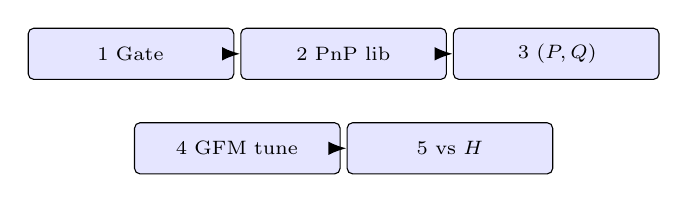
\begin{tikzpicture}
  \node[ColA, text width=2.4cm] (w1) at (0,0) {1 Gate};
  \node[ColA, text width=2.4cm] (w2) at (2.7,0) {2 PnP lib};
  \node[ColA, text width=2.4cm] (w3) at (5.4,0) {3 $(P,Q)$};
  \node[ColA, text width=2.4cm] (w4) at (1.35,-1.2) {4 GFM tune};
  \node[ColA, text width=2.4cm] (w5) at (4.05,-1.2) {5 vs $H$};
  \draw[Narr] (w1)--(w2);
  \draw[Narr] (w2)--(w3);
  \draw[Narr] (w4)--(w5);
\end{tikzpicture}
\end{center}

Gate $\to$ catalog; $(P,Q)$ / OPF region; droop search; local-vs-$H$.

%==============================================================================
\section{End-to-end flowchart}
%==============================================================================

\begin{center}
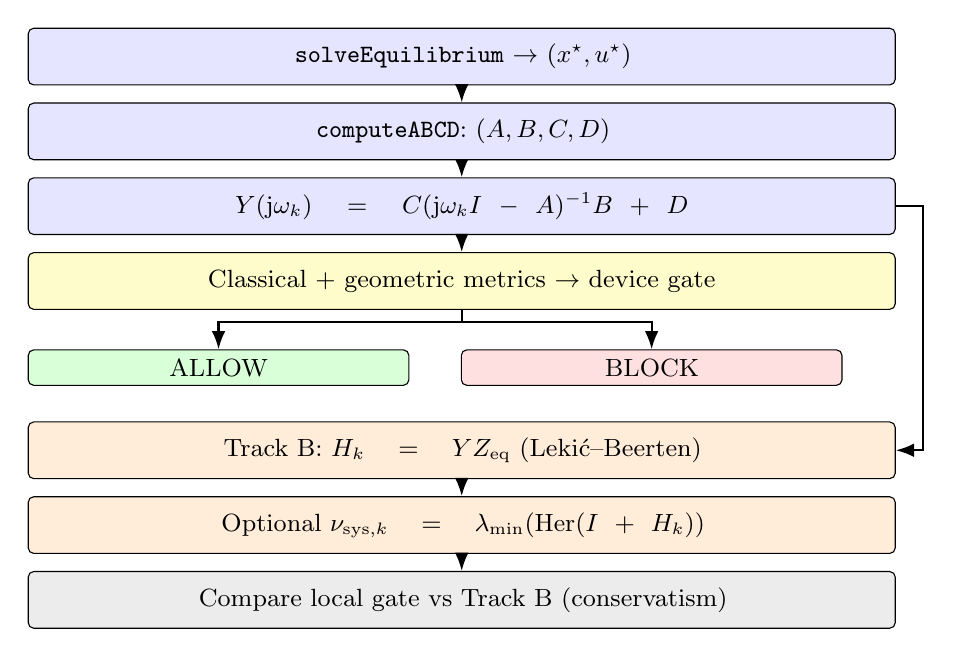
\begin{tikzpicture}
  \node[Fbox, fill=blue!10, text width=10.8cm] (eq) at (0,0)
    {\code{solveEquilibrium} $\to$ $(x^\star,u^\star)$};
  \node[Fbox, fill=blue!10, text width=10.8cm] (abcd) at (0,-0.95)
    {\code{computeABCD}: $(A,B,C,D)$};
  \node[Fbox, fill=blue!10, text width=10.8cm] (Y) at (0,-1.9)
    {$Y(\jomega_k)=C(\jomega_k I-A)^{-1}B+D$};
  \node[Fbox, fill=yellow!20, text width=10.8cm] (met) at (0,-2.85)
    {Classical + geometric metrics $\to$ device gate};

  \node[draw, rounded corners=2pt, fill=green!15, text width=4.6cm,
        align=center, font=\small, anchor=west] (ok) at (0,-3.95) {ALLOW};
  \node[draw, rounded corners=2pt, fill=red!12, text width=4.6cm,
        align=center, font=\small, anchor=west] (bad) at (5.5,-3.95) {BLOCK};

  \node[Fbox, fill=orange!15, text width=10.8cm] (H) at (0,-5.0)
    {Track B: $H_k=YZ_{\mathrm{eq}}$ (Leki\'c--Beerten)};
  \node[Fbox, fill=orange!15, text width=10.8cm] (sys) at (0,-5.95)
    {Optional $\nu_{\mathrm{sys},k}=\lambda_{\min}(\Her(I+H_k))$};
  \node[Fbox, fill=gray!15, text width=10.8cm] (cmp) at (0,-6.9)
    {Compare local gate vs Track B (conservatism)};

  \draw[Narr] (eq.south)--(abcd.north);
  \draw[Narr] (abcd.south)--(Y.north);
  \draw[Narr] (Y.south)--(met.north);
  \draw[Narr] (met.south) -- ++(0,-0.15) -| (ok.north);
  \draw[Narr] (met.south) -- ++(0,-0.15) -| (bad.north);
  \draw[Narr] (H.south)--(sys.north);
  \draw[Narr] (sys.south)--(cmp.north);
  \draw[Narr] (Y.east) -- ++(0.35,0) |- (H.east);
\end{tikzpicture}
\end{center}

%==============================================================================
\section{How to run tests}
%==============================================================================

\subsection{Unit tests (GoogleTest)}
Source: \code{tests/testCertificate.cpp}. Executable: \code{testharmony}
(from the \code{tests/} CMake project).

\begin{center}
\renewcommand{\arraystretch}{1.2}
\begin{tabularx}{\textwidth}{@{}L{2.4cm} Y@{}}
\toprule
Suite & Covers (GTest filter) \\
\midrule
Metrics
& Classical $\nu$, shifted passivity
(\texttt{CertificateMetrics.*}). \\
Workflows
& Device gate + PnP JSON; sweep sizes
(\texttt{CertificateWorkflows.*}). \\
Geometric
& NR / DW-lite / small-gain / sector
(\texttt{GeometricCertificates.*}). \\
\bottomrule
\end{tabularx}
\end{center}

\begin{lstlisting}
testharmony.exe --gtest_filter=GeometricCertificates*
testharmony.exe --gtest_filter=Certificate*:GeometricCertificates*
\end{lstlisting}

\subsection{Integration / paper demo}
\begin{lstlisting}
Harmony --cpp certificate_figures --no-plot
Harmony --cpp certificate_figures
\end{lstlisting}
Expected on default GFM-MMC: local \textbf{BLOCK} (passivity FAIL);
system $\Her(I+H)$ \textbf{PASS}; verdict \textbf{DISAGREE}.

Smoke test: \code{testexamples.cpp} calls
\code{example_certificate_figures(false)}.

%==============================================================================
\section{Distinctive test cases vs classical Beerten studies}
%==============================================================================

Classical Beerten / early MMC impedance papers emphasized averaged MMC models,
GFL-oriented controls, and impedance / eigenvalue / EMT validation of $H$ ---
not decentralized geometric gates, GFM droop certificates, post-OPF $(P,Q)$
regions, or open multi-case toolbox packs.

\subsection{Cases Harmony / CRESYM can uniquely offer}

\begin{center}
\renewcommand{\arraystretch}{1.2}
\begin{tabularx}{\textwidth}{@{}L{3.5cm} Y@{}}
\toprule
Case family & What is new \\
\midrule
GFM-MMC + local vs $H$
& Outer-loop GFM; passivity/NR FAIL vs $H$ PASS table.
Demo: \code{certificate_figures}. \\
Non-passivity band maps
& Contours of $\nu(f)$, $\nu_-(f)$, $\varphi_{\mathrm{NR}}(f)$,
$\nu(P,Q)$, $\nu(K_P,K_Q)$; overlay $H$-margins. \\
Post-OPF certified $(P,Q)$
& OPF setpoint + certificate region around $(P^\star,Q^\star)$. \\
MTDC / multi-MMC PnP
& ALLOW/BLOCK catalog; recheck gates vs $H$ at each cut. \\
AC/DC multiport cuts
& Certify $Y_{\mathrm{aa}}$, $Y_{\mathrm{dd}}$, full $Y$; AC and DC $H$. \\
Weak AC / topology
& SCR / topology sweeps: when local geometry disagrees with $H$. \\
Open reproducible pack
& JSON/C++ cases + CSV sweeps (software-paper asset). \\
EMT / RTDS twin
& Contested OPs where PnP blocks but $H$ passes. \\
\bottomrule
\end{tabularx}
\end{center}

\subsection{Minimal paper case pack}
\begin{enumerate}[leftmargin=*,itemsep=0.15em]
  \item \textbf{C0} Stiff-grid GFM-MMC (\code{mmc_gfm} /
        \code{certificate_figures}) --- baseline disagreement.
  \item \textbf{C1} Same MMC, weak SCR sweep (e.g.\ SCR $=2$--$10$).
  \item \textbf{C2} Point-to-point HVDC with AC and DC $H$ cuts.
  \item \textbf{C3} Three-terminal MTDC: add/remove one converter.
  \item \textbf{C4} OPF-feasible $(P,Q)$ cloud + certificate overlay.
  \item \textbf{C5} (optional) EMT check of 2--3 contested points.
\end{enumerate}

%==============================================================================
\section{Literature map}
%==============================================================================

\textbf{Passivity / phase:} excess passivity, small-phase, numerical range;
He--D\"orfler dVOC passivity (TPWRS).

\textbf{GFM parametric PnP / loop-shifting:}
H\"aberle--He--Huang--D\"orfler--Low, arXiv:2503.05403;
dynamic multipliers arXiv:2602.09150.

\textbf{DW-shell / SRG (full interconnection):}
arXiv:2508.17033; arXiv:2507.19918;
Baron-Prada--Anta--D\"orfler SRG arXiv:2601.16014.

\textbf{IQC / multipliers:} IQC, Zames--Falb, dissipativity.

\textbf{Track B:} Leki\'c--Beerten / Sakinci--Leki\'c--Beerten
$H=YZ_{\mathrm{eq}}$ --- gold-standard comparator.

\textbf{Expansion order:}
(1)~NR/DW-lite conservatism on C0--C1 vs $H$;
(2)~weaker local rules on non-passivity bands;
(3)~full network DW/SRG only if compositional PnP claims are required;
(4)~always validate vs $H$.

%==============================================================================
\section{GFM non-passivity bands (theory target)}
%==============================================================================

\[
  \Omega_{\mathrm{bad}}=\{\omega:\nu(Y_{\mathrm{ac}}(\jomega))<\varepsilon\}.
\]
Seek property $C$ on $\Omega_{\mathrm{bad}}$ such that
$C(Y)$ + network class $\mathcal{Z}$ implies interconnection OK
(consistent with $H$/Nyquist). Geometric metrics already expose
$\nu_-$, $\varphi_{\mathrm{NR}}$, and $m_0$ over frequency for this programme.

%==============================================================================
\section{Regenerate evidence}
%==============================================================================

\begin{lstlisting}
Harmony --cpp certificate_figures
Harmony --cpp certificate_figures --no-plot
Harmony --cpp mmc_gfm
testharmony.exe --gtest_filter=GeometricCertificates*
\end{lstlisting}

Outputs under \code{files/}: sweeps (incl.\ NR phase, zero-margin, small-gain,
shortage), operating-region CSV, PnP library JSON.

%==============================================================================
\section{Symbol table}
%==============================================================================

\begin{center}
\renewcommand{\arraystretch}{1.1}
\begin{tabularx}{\textwidth}{@{}L{2.4cm} Y@{}}
\toprule
Symbol & Meaning \\
\midrule
$Y$ & Device terminal admittance \\
$Y_{\mathrm{ac}}$ & AC $dq$ block \\
$\nu$ & $\lambda_{\min}(\Her Y)$ \\
$\nu_+,\nu_-$ & excess / shortage passivity \\
$\varphi_{\mathrm{eig}}$ & max eigenphase (heuristic) \\
$\varphi_{\mathrm{NR}}$ & numerical-range phase (small-phase) \\
$W(Y)$ & numerical range / field of values \\
$m_0$ & NR zero-margin ($>0\Rightarrow 0\notin W$) \\
$\sigma_{\max}$ & operator norm (small-gain) \\
$\mathrm{DW}(Y)$ & Davis--Wielandt shell \\
$Z_{\mathrm{eq}}$ & Network equivalent at cut \\
$H$ & $YZ_{\mathrm{eq}}$ (Leki\'c--Beerten) \\
$\nu_{\mathrm{sys}}$ & $\lambda_{\min}(\Her(I+H))$ proxy \\
\bottomrule
\end{tabularx}
\end{center}

\end{document}
